\graphicspath{{chapters/07/images/}}
\chapter{Introduction}

\subsection{Definition of a system}
A system is a set of integrated and interacting \emph{components} or \emph{entities} that form a whole with definite boundaries and surrounding environment.
A system has a goal to achieve by performing one or more functions or tasks.
Systems can be aggregated into a \textbf{\emph{hierarchy}}.
A system at a given level of detail can be a component at a higher level of detail.

\begin{itemize}
\item A \textbf{\emph{complex}} (non-linear) \textbf{\emph{system}} is a system that does not satisfy the principle of superposition, i.e., the behavior of the system cannot be inferred from the behavior of its components.
\item A \textbf{\emph{dynamical system}} is a system where fixed rules define the time dependencies of the system in a geometrical space.
  Dynamical systems have a space and time dimension because they change their characteristics over time.
  If we pick snapshots of the system at different time points, we observe different configurations of the system (data).
\end{itemize}
\noindent
A \textbf{\emph{configuration}} or state of the system refers to the current condition of the system and stores enough information to predict its next move.
A state is characterized by the position of its components in a geometrical space and by the values of the attributes of its components (e.g., concentration or number of each elements involved).
Systems change their state over time by changing the location of some of their components or changing the attributes of some of their components.

\begin{itemize}
  \item \textbf{\emph{steady state}}: some of the attributes of the system are no longer changing in the future.
  \item \textbf{\emph{transient state}}: time needed to reach the steady state.
\end{itemize}


\subsection{Determinism, nondeterminism, or stochasticity?}

\begin{itemize}
\item
  \textbf{\emph{Deterministic systems}} always react in the same way to
  the same set of stimuli. These systems are completely determined by
  the initial state and the input set. The essence of deterministic
  systems is that each event is causally related to previous events and
  choices are always resolved in the same way in the same context. When
  a system generates multiple outcomes from the same input in different
  observations, the system is \textbf{\emph{nondeterministic}} (we
  cannot predict the output from the input).
\item
  \textbf{\emph{Stochasticity}} is the quality of lacking any
  predictable order or plan and stochastic systems possess some inherent
  randomness. It is possible to transform a nondeterministic system into
  a stochastic one by attaching probabilities to the selection points so
  that we turn nondeterministic choices into probabilistic choices.
\end{itemize}


\subsection{Computational complexity}

Complexity arises when interacting components self-organize to form
evolving structures that exhibit a hierarchy of emergent system
properties. An \textbf{\emph{emergent behavior}} can be originated by a
collection of components that interact in the absence of a centralized
point of control to produce something that has not been designed or
programmed in the system construction or evolution. Example: internet,
ant colonies, consciousness.\\
\\
\noindent
\textbf{\emph{Computational complexity}} is the amount of resources,
measured as a function of the size of the input, needed to execute an
algorithm.

\begin{itemize}
\tightlist
\item
  Computational space complexity: the amount of memory needed;
\item
  Computational time complexity: the number of instructions to be
  executed.
\end{itemize}


\subsection{Definition of a model}

A \emph{representation} is a set of symbols used to convey information
and knowledge about a system. It is either physical as a cell or an
ecosystem, or artificial as a computer network or an economic market. An
abstraction is a representation that ignores some aspects of a system
which are not of interest for the current investigation.
\\
\\
\noindent
A \emph{model} is an abstraction of a system. A model has its own interacting
components that are characterized by the attributes that we want to
observe. The set of all the attributes in a model is the
\emph{experimental frame}.

\begin{itemize}
\item
  A \emph{dynamic model} aims at predicting the behavior of the system
  in time/space through what if analysis. \textbf{What if analysis} investigates
  how a change in some attributes affects the behavior of the modeled
  system.
\item
  A \emph{computational model} is a model that can be manipulated by a
  computer to observe properties of the corresponding system.

  \begin{figure}
  \centering
  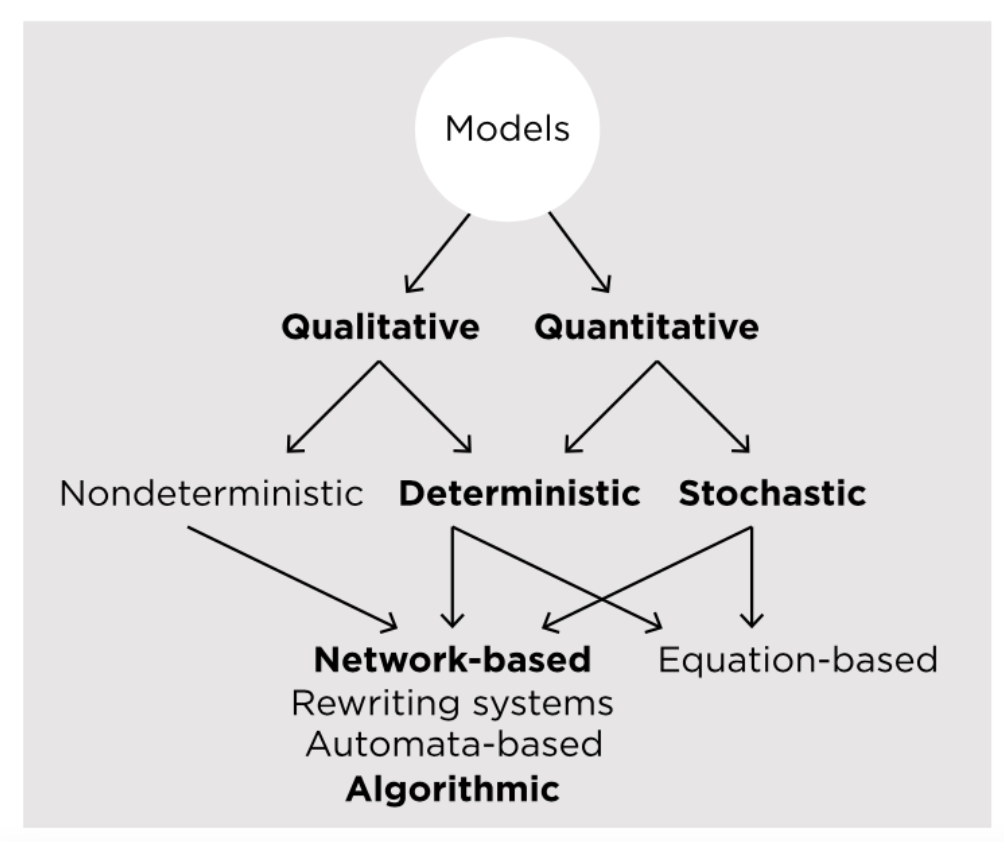
\includegraphics[width=0.6\textwidth]{scheme_model.png}
  \caption{From a model to methods}
  \end{figure}
\end{itemize}


\subsection{Checking the validity of a model}

\emph{Validity} is a fundamental property of models and witnesses the
capacity of a model of making good predictions. We need to assess the validity of a
model before using it to predict the behavior of a system.
\\
\\
\noindent
Assume that $M$ is a model for the system $S$ and $\underline{M}$ is the
modeling process. Let $s(t)$ and $m(t)$ be the state of the system and
of the model at time $t$, and $f_s$ and $f_m$ the state transition
functions of the system and of the model, respectively. Finally, let
$I_s(t)$ and $O_s(t)$ be the input and output of the system at time $t$.
Similarly, we write $I_m(t)$ and $O_m(t)$ for the model.
\\
\\
\noindent
What we expect is that going from one state to the other we have a
function (one for the system and one for the model); in a mathematical
model we integrate the $f_m$ function to known what happens in the
transition of the model, but we cannot do that in the real setting (the
transition function $f_s$ is not known) → when dealing with nature, we
cannot validate models according to the previous definition, so we use
I/O validity, based on known input and outputs of the system.
\\
\\
\noindent
The input and output are here generalized concepts: input can be any
perturbation of the system or of the model, and output can be any
observable property causally related to the input.
\\
\\
\noindent
A model $M$ is valid for a system $S$ if:
$f_m(\underline{M}(s(t_0))) = \underline{M}(f_s(s(t_0))) = m(t_1)$

\begin{figure}
\centering
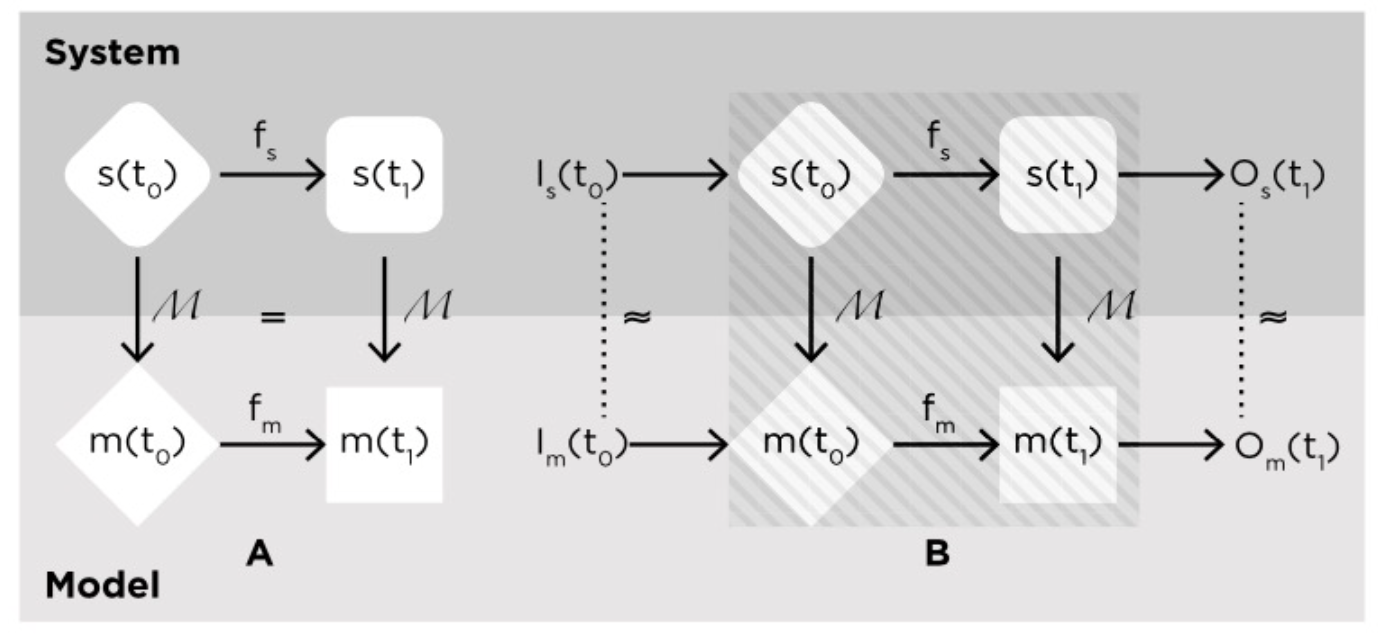
\includegraphics[width=0.7\textwidth]{validation.png}
\caption{validation}
\end{figure}
\noindent
I/O validity can be checked by using data sets produced by the model and
observed and measured on the system. An issue in this comparison process
is \emph{overfitting}:

\begin{itemize}
\tightlist
\item
  a model is well tuned to a specific dataset used to build the model
\item
  it performs poorly on other datasets
\end{itemize}
\noindent
\textbf{Cross-validation}: check overfitting by testing the model on
data sets different from the ones used to build and calibrate/train the
model.
\\
\\
\noindent
These concepts, even if usually referred to computational models, may
apply to general models or representations of a system.


\subsection{How to build a model}

We need to define objectives:

\begin{itemize}
\tightlist
\item
  what do you want to model?
\item
  what do you want to investigate with the model?
\item
  what do you expect from the model?
\item
  why do you need a model?
\end{itemize}

\begin{figure}
\centering
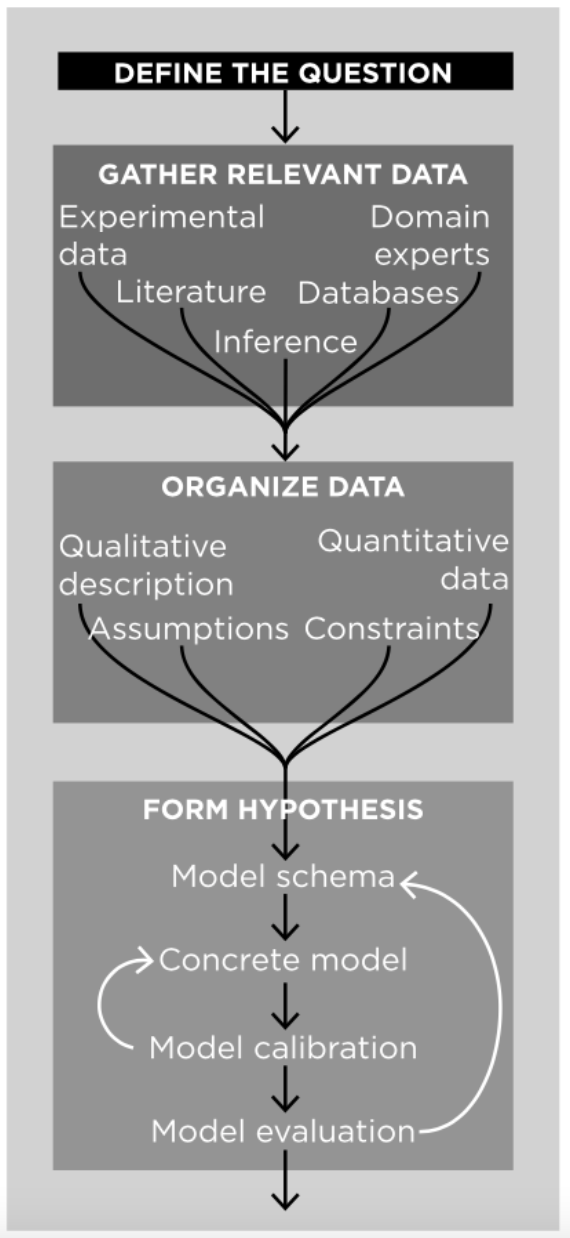
\includegraphics[width=0.3\textwidth]{workflow.png}
\caption{Workflow}
\end{figure}

\noindent
After defining the question and gathering data, we need to build the
model and calibrate it, in order to check if it can recapitulate data.
If it does not, either we are missing something or we must tune some
parameters. Different parameters can lead to dramatic changes in
dynamics. Example: Lotka-Volterra model with different parameter
conditions (Figure \ref{fig:Volterra}).

\begin{figure}
\centering
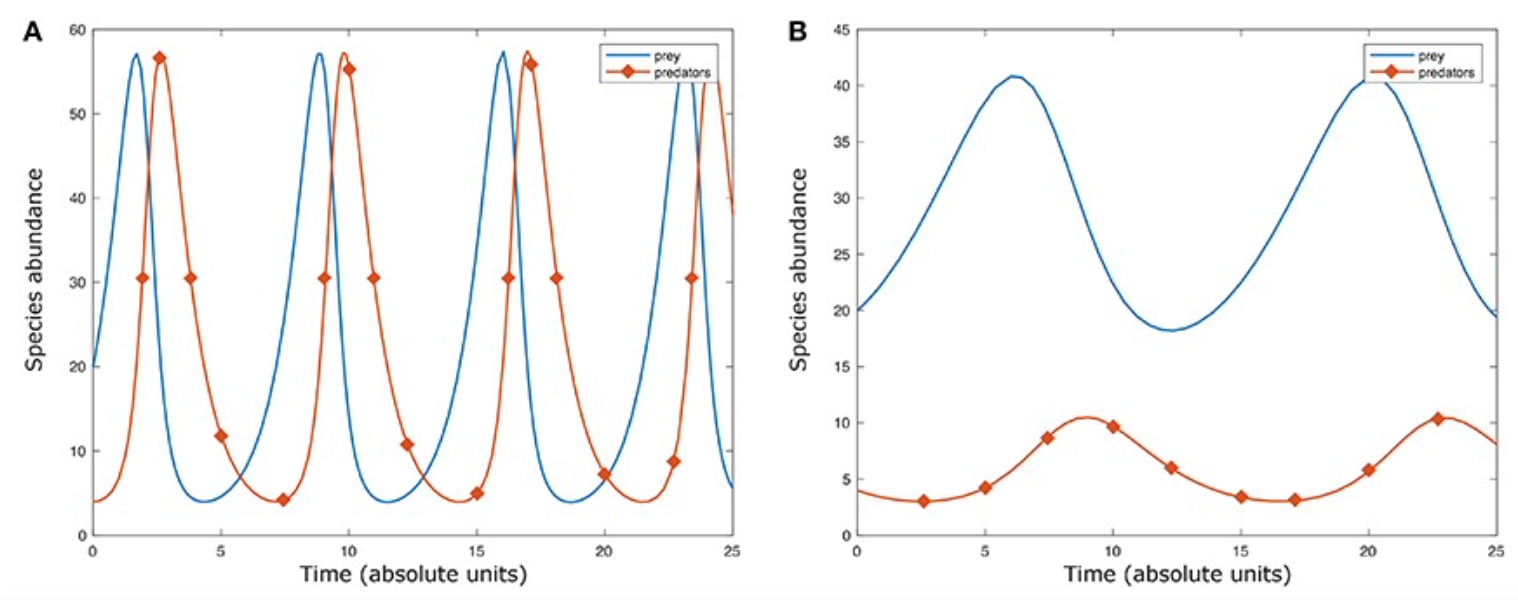
\includegraphics[width=\textwidth]{volterra.png}
\caption{Volterra}
\label{fig:Volterra}
\end{figure}

\begin{enumerate}
\def\labelenumi{\Alph{enumi})}
\item
  shows periodic oscillations, same amount of preys and predators
\item
  wider peaks and lower predator presence
\end{enumerate}
